
\subsection{Reactant hierarchy}

\begin{figure}[!h]
  \centering
  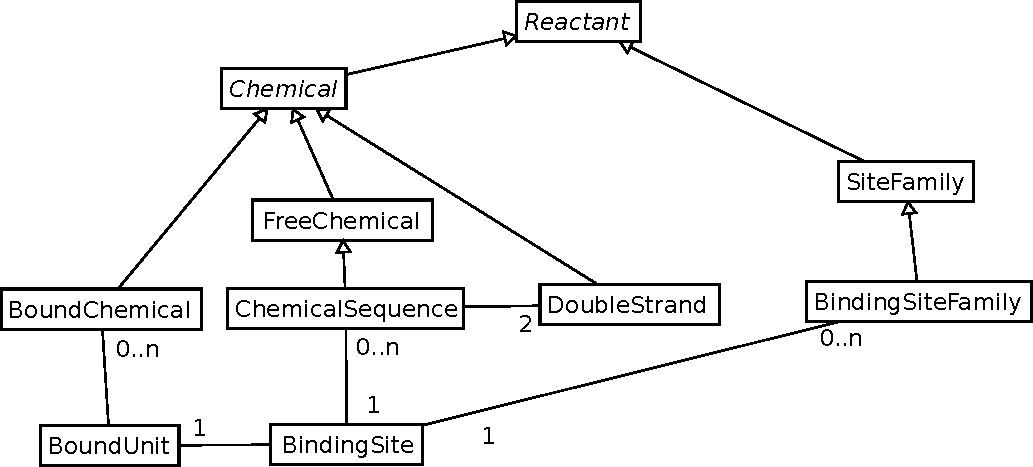
\includegraphics[width=0.8\linewidth]{reactant_uml}
  \caption{UML diagram of \texttt{Reactant} hierarchy}
  \label{fig:reactant_uml}
\end{figure}

The following sections give a quick overview of the contents of the \texttt{Reactant} hirarchy~\reffigp{fig:reactant_uml}. More details about how reactants are implemented can be found later.

\subsubsection{Reactant}

\texttt{Reactant} is a global abstract interface. All entities that can participate in a reaction \emph{must} inherit from it.

\subsubsection{Chemical}

\begin{figure}[!h]
  \centering
  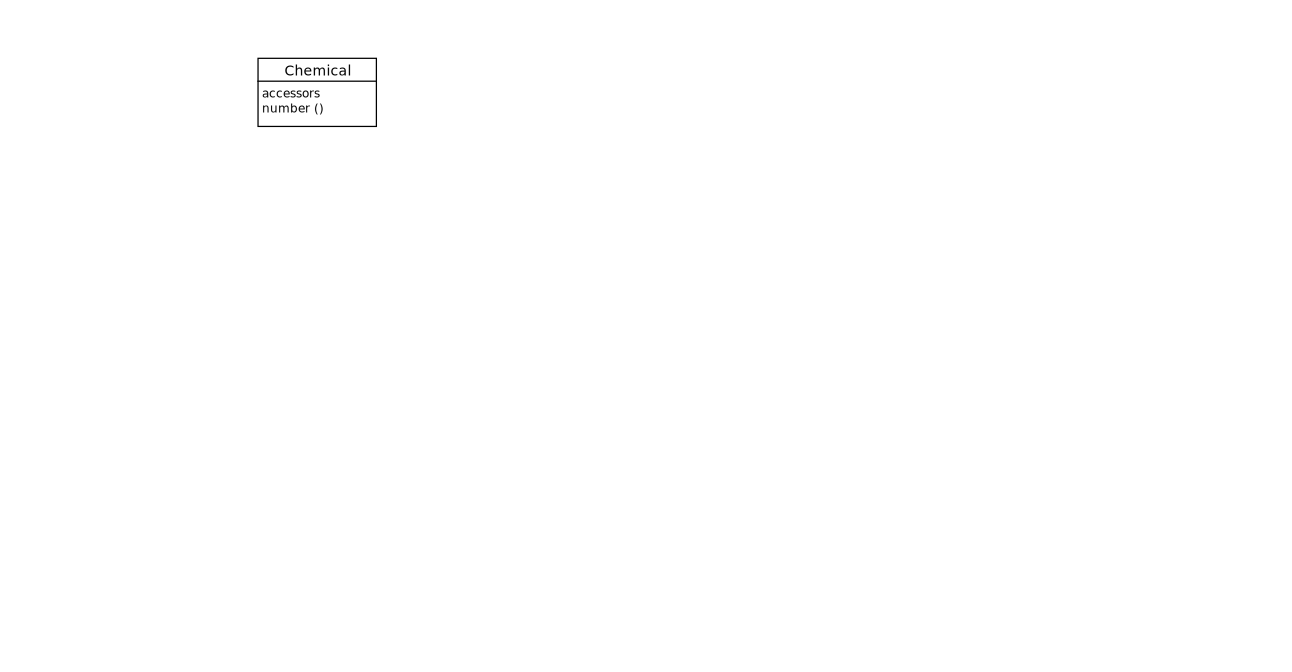
\includegraphics[scale=0.8]{chemical}
  \caption{\texttt{Chemical} class}
  \label{fig:chemical}
\end{figure}

\texttt{Chemical} is an abstract class~\reffigp{fig:chemical}. It defines all standard chemical entities. \texttt{Chemical} represents a \emph{pool} of a given chemical species, meaning that one may access its current number at any time.

\subsubsection{FreeChemical}

\paragraph{Input format}
\begin{verbatim}
FreeChemical <name> [<initial quantity>]
\end{verbatim}

\begin{figure}[!h]
  \centering
  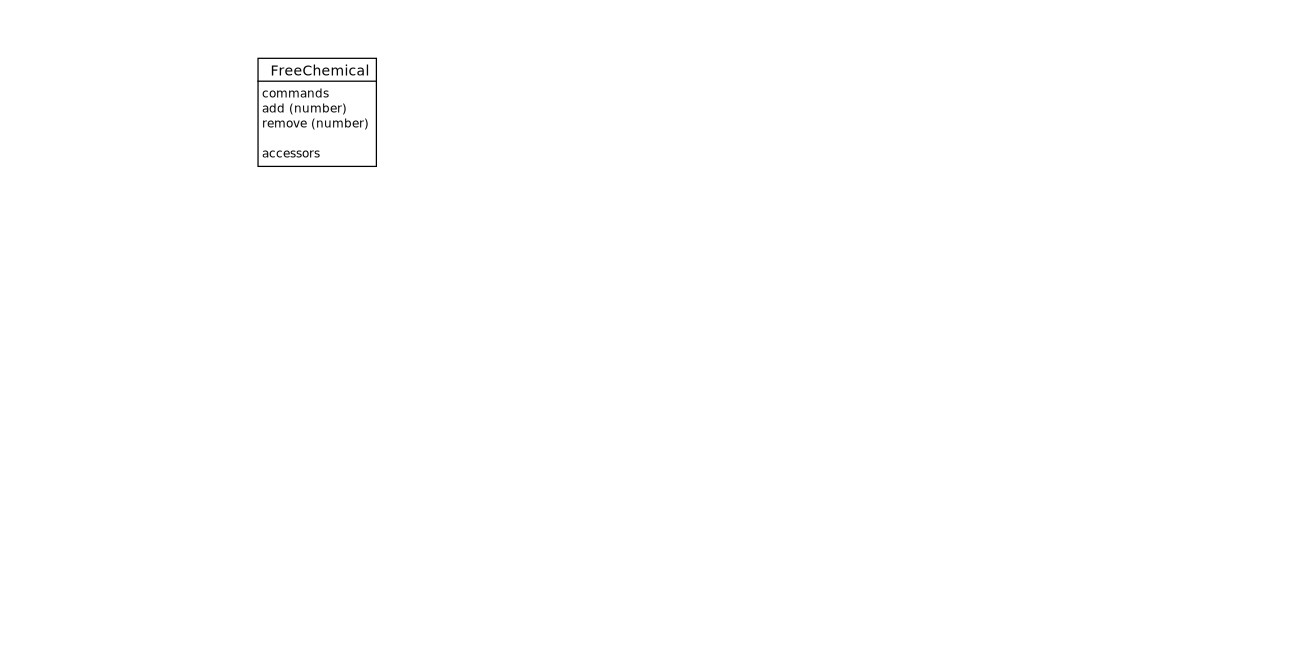
\includegraphics[scale=0.8]{freechemical}
  \caption{\texttt{FreeChemical} class}
  \label{fig:free_chemical}
\end{figure}

\texttt{FreeChemical}~\reffigp{fig:free_chemical} is a subclass of \texttt{Chemical} that represents free chemical (\textit{e.g.} molecules diffusing in the cytosol or extracellular medium).

\subsubsection{BoundChemical}

\paragraph{Input format}
\begin{verbatim}
BoundChemical <name>
\end{verbatim}

\begin{figure}[!h]
  \centering
  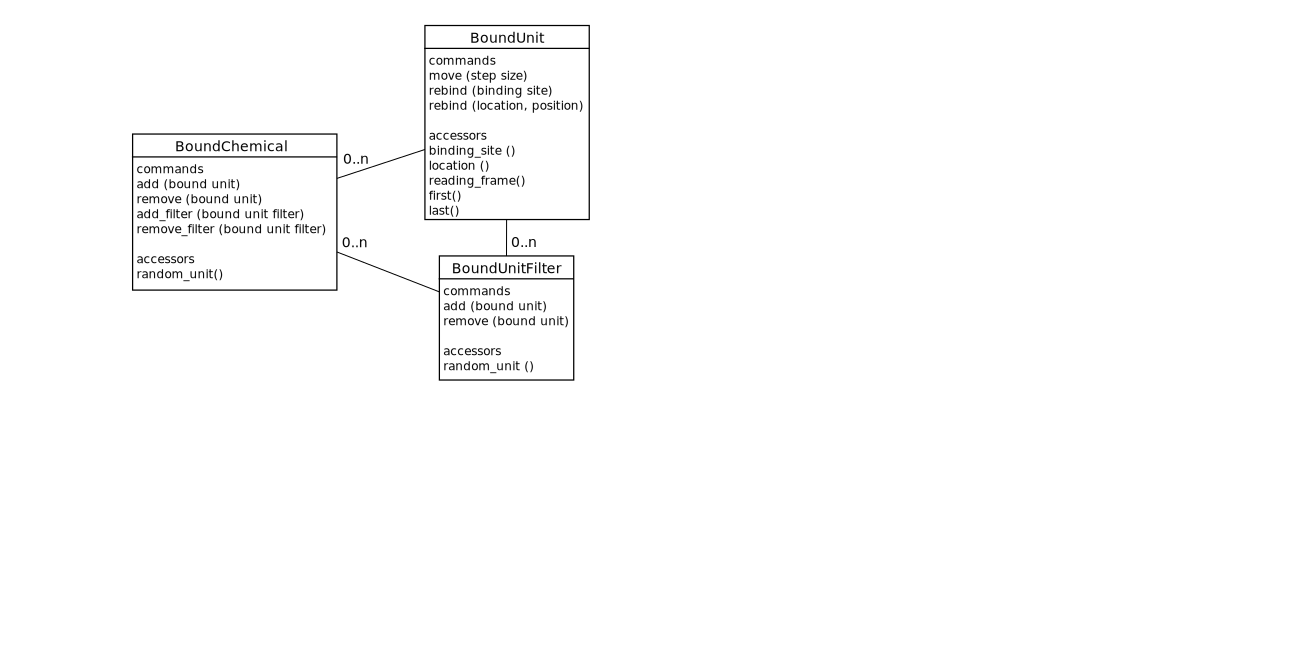
\includegraphics[scale=0.8]{boundchemical}
  \caption{\texttt{BoundChemical} class}
  \label{fig:bound_chemical}
\end{figure}

\texttt{BoundChemical}~\reffigp{fig:bound_chemical} is a subclass of \texttt{Chemical} that represents chemicals that are bound to a sequence. It is important to note it only represents molecules bound to the sequence, \emph{not} the complex formed by the chemical and the sequence. Even though \texttt{BoundChemical} represents a pool of molecules, single elements are not interchangeable, they are defined by their position on a sequence. \texttt{BoundChemical} uses class \texttt{BoundUnit} to represent molecules individually. It uses \texttt{BoundUnitFilter} to organize bound units according to outside criteria needed for reactions (classify according to binding sites, motifs read, etc.). It also uses \texttt{Switch}es on specific switch sites that are sequence dependent (this will be explained in detail later).

\subsubsection{ChemicalSequence}

\paragraph{Input format}
\begin{verbatim}
ChemicalSequence <name> sequence <sequence> [<initial quantity>]
TransformationTable <name> [<parent_letter> <product_letter>,]^{1..n}
ProductTable <name> <transformation table>
ChemicalSequence <name> product_of <parent sequence> \
  <starting position> <ending position> <product table> [<initial quantity>]
\end{verbatim}

\begin{figure}[!h]
  \centering
  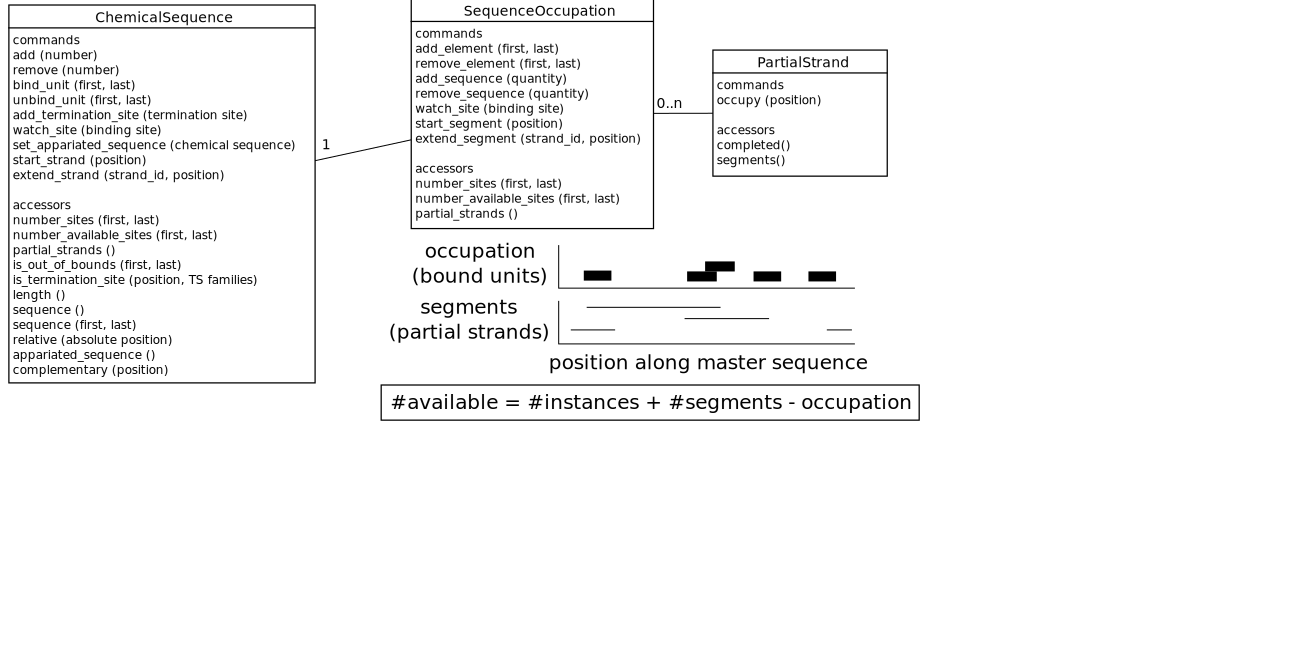
\includegraphics[scale=0.7]{chemicalsequence}
  \caption{\texttt{ChemicalSequence} class}
  \label{fig:chemical_sequence}
\end{figure}

\texttt{ChemicalSequence}~\reffigp{fig:chemical_sequence} is a subclass of \texttt{FreeChemical}. It is defined by a sequence and the ability to bind elements. However, instances of a sequence are \emph{not} treated individually, it is impossible to tell to which instance a given chemical bound. An object called \texttt{SequenceOccupation} maintains occupation levels at sites of interest. For example, suppose the sequence is an mRNA carrying a ribosome binding site for the protein DnaA. The number of available sites is obtained by removing the number of bound chemicals occupying the site from the number of instances of the mRNA currently in the cell. A \texttt{ChemicalSequence} can be appariated to another \texttt{ChemicalSequence}. A \texttt{ChemicalSequence} can be created from a sequence or as a product of another sequence, in which case a \texttt{TransformationTable} is needed to generate the product's sequence from the parent's, and a \texttt{ProductTable} stores the parent/product relationship.

\subsubsection{DoubleStrand}

\paragraph{Input format}
\begin{verbatim}
TransformationTable <name> [<letter> <complementary_letter>,]^{1..n}
DoubleStrandSequence <name> <name_sense_sequence> <sense_sequence> \
  <name_antisense_sequence> <transformation_table> [<initial quantity>]
\end{verbatim}

\begin{figure}[!h]
  \centering
  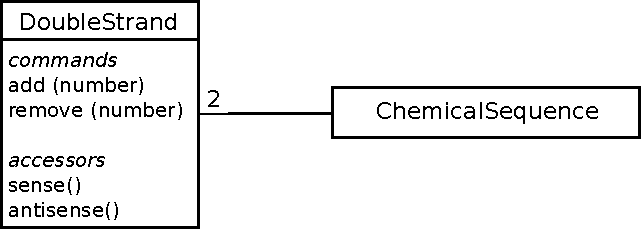
\includegraphics[scale=0.8]{doublestrand}
  \caption{\texttt{DoubleStrand} class}
  \label{fig:double_strand}
\end{figure}

\texttt{DoubleStrand}~\reffigp{fig:double_strand} links two \texttt{ChemicalSequence} together that are biochemically linked (\textit{e.g.} DNA), one sequence being complementary to the other. It enables segment extension on the appariated strand and free end binding (see interface of \texttt{ChemicalSequence}). A \texttt{DoubleStrand} is created from a sense sequence that is specified similarly to a \texttt{ChemicalSequence}. However, the complementary sequence is created from a \texttt{TransformationTable} that specifies how to transform the sense sequence into antisense sequence (\textit{e.g.} for DNA, $A\rightarrow T$, $T\rightarrow A$, $C\rightarrow G$, $G\rightarrow C$).

\subsubsection{BindingSiteFamily}

\begin{figure}[!h]
  \centering
  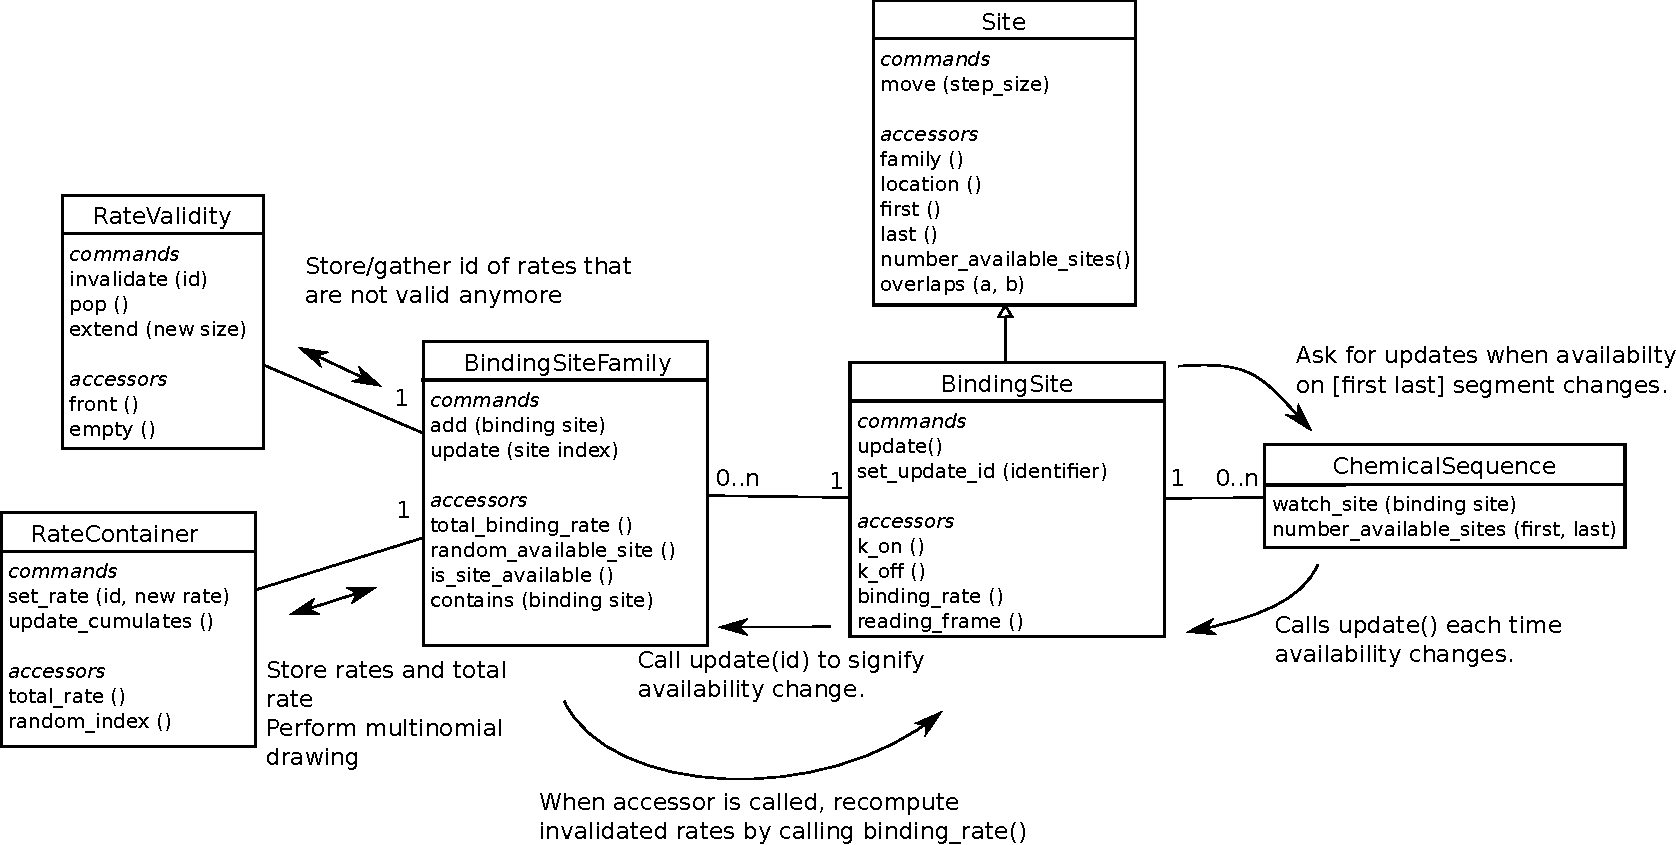
\includegraphics[scale=0.8]{bindingsitefamily}
  \caption{\texttt{BindingSiteFamily} class}
  \label{fig:bsf}
\end{figure}

\texttt{BindingSiteFamily}~\reffigp{fig:bsf} is a subclass of \texttt{Reactant}. Contrary to \texttt{Chemical}, it does not represent a countable pool of molecules. Each family contains a number of related instances of \texttt{BindingSite} (\textit{e.g.} ribosome binding sites). \texttt{BindingSiteFamily}, \texttt{BindingSite} and \texttt{ChemicalSequence} use a notification pattern (via \texttt{update} methods) to dynamically maintain the number of available sites for each binding site as well as binding rates up to date. If a binding site is used to load polymerases, a reading frame should be provided to specify where a polymerase will start reading the sequence after binding.

\paragraph{Input format}
\begin{verbatim}
BindingSite <binding site family name> <chemical sequence> \
  <start> <end> <k_on> <k_off> [<reading frame>]
\end{verbatim}
